\documentclass[tikz, border=5pt]{standalone}
\usepackage{xstring}
\usetikzlibrary{decorations.pathreplacing,
positioning}

\newcommand{\GetBit}[2]{%
    \edef\BitPos{#2}%
    \StrLen{#1}[\StringLen]%
    \StrChar{#1}{#2}[\Bit]%
}
\newcommand{\SetBits}[2]{%
    \foreach \i in {1,...,#2} {%
            \GetBit{#1}{\i}%
            \node at (\i - 0.5, 0.5) {\LARGE \textbf{\Bit}};
        }%
}
\newcommand{\drawBraceLabel}[4]{%
    \draw [decorate, decoration={brace, amplitude=5pt}] (#1, -0.1) -- (#2, -0.1);
    \node [below] at (#3, -0.3) {\parbox{3cm}{\centering\texttt{#4}}};
}

\begin{document}
\begin{tikzpicture}

    % Colors
    \fill [gray!10] (0, 0) rectangle (32, 1);
    \fill [red!10] (11, 0) rectangle (12, 1);
    \fill [blue!10] (14, 0) rectangle (16, 1);
    \fill [cyan!10] (18, 0) rectangle (19, 1);
    \fill [green!10] (19, 0) rectangle (24, 1);
    \fill [yellow!20] (30, 0) rectangle (32, 1);

    % Boxes
    \foreach \i in {0,...,31} {
            \draw (\i, 0) rectangle (\i + 1, 1);
        }
    \SetBits{00000000000E00DD00CBBBBB000000AA}{32}

    % Labels
    \drawBraceLabel{16-0.025}{14+0.025}{15}{POLARITY}
    \drawBraceLabel{19-0.025}{18+0.025}{18.5}{PORT}
    \drawBraceLabel{24-0.025}{19+0.025}{21.5}{PSEL}
    \drawBraceLabel{32-0.025}{30}{31}{MODE}

    % Positions
    \foreach \i in {0,...,31} {
            \node [above] at ({31.5 - \i}, 1) {\texttt{\number\numexpr\i}};
        }

\end{tikzpicture}
\end{document}
